% TikZ + pgfplots: the canonical "the AST must not touch this" content.
\documentclass{standalone}
\usepackage{tikz}
\usepackage{pgfplots}
\pgfplotsset{compat=1.18}
\usetikzlibrary{arrows.meta,positioning,calc,decorations.pathmorphing}
\usepgfplotslibrary{groupplots}

\begin{document}

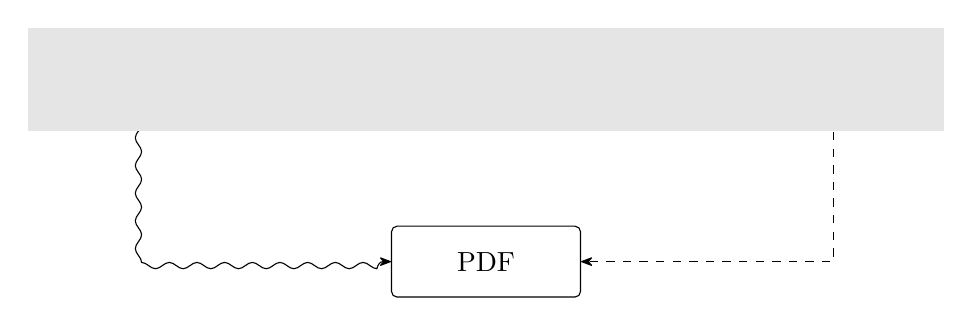
\begin{tikzpicture}[
    node distance=1.4cm and 2cm,
    block/.style={draw, rounded corners=2pt, minimum width=2.4cm, minimum height=0.9cm},
    >={Stealth[round]}
  ]
  \node[block] (src)  {Source};
  \node[block, right=of src] (parse) {Parser};
  \node[block, right=of parse] (ast)  {AST};
  \node[block, below=of parse] (pdf)  {PDF};

  \draw[->] (src)   -- node[above,font=\small] {text} (parse);
  \draw[->] (parse) -- node[above,font=\small] {nodes} (ast);
  \draw[->, dashed] (ast) |- (pdf);
  \draw[->, decorate, decoration={snake, amplitude=.4mm}] (src) |- (pdf);

  \fill[gray!20] ($(src.south west) + (-0.2,-0.2)$) rectangle ($(ast.north east) + (0.2,0.2)$);
\end{tikzpicture}

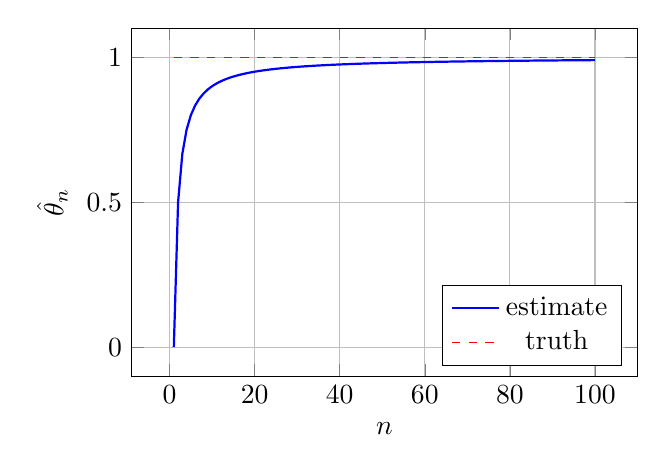
\begin{tikzpicture}
  \begin{axis}[
      width=8cm, height=6cm,
      xlabel={$n$}, ylabel={$\hat\theta_n$},
      grid=major, legend pos=south east,
    ]
    \addplot[blue, thick, domain=1:100, samples=100] {1 - 1/x};
    \addlegendentry{estimate}
    \addplot[red, dashed, domain=1:100] {1};
    \addlegendentry{truth}
  \end{axis}
\end{tikzpicture}

\end{document}
